\section{}
Per controllare un display con una vga serve sapere delle cose

\subsection{Preliminari}
Bisogna conoscere il framerate dello schermo, ovvero la quantit\`a di volte al secondo in cui viene disegnata l'immagine su di esso. Per ogni frame visualizzato lo schermo per un certo periodo rimane nero, bisogna tenere conto di questo vuoto con un parametro detto \textbf{retrace factor}. Infine bisogna aver presente la risoluzione dello schermo (ad esempio $1280\times1024$).

Con questi parametri si calcola il pixelclock, ovvero la frequenza con cui vengono mandate le informazioni allo schermo:
\begin{equation}\label{eq:pixelclock}
PixelClock = \frac{(Horiz\ Res) \times (Vert\ Res) \times (Frame\ Rate)}
{Retrace Factor}
\end{equation}

\subsection{Un frame}
Ora cercher\`o di descrivere come funziona un frame, poi Alex legger\`a e corregger\`a.

\begin{figure}[hbt]
	\centering
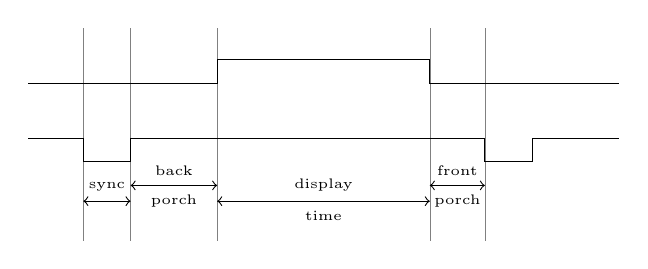
\begin{tikzpicture}
\def	\fp	{0.7};
\def	\bp	{1.1};
\def	\s	{0.6};
\def	\d	{2.7};
\def	\h	{0.3};
\def	\hb	{2.7};
\begin{scope}[help lines]%[gray,ultra thin]
\draw (\fp,-2)--++(0,\hb);
\draw (\fp+\s,-2)--++(0,\hb);
\draw (\fp+\s+\bp,-2)--++(0,\hb);
\draw (\fp+\s+\bp+\d,-2)--++(0,\hb);
\draw (\fp+\s+\bp+\d+\fp,-2)--++(0,\hb);
\end{scope}
\begin{scope}[<->]
\draw (\fp,-1.5) --+ (\s,0) node [sloped,midway,above] {\tiny sync};
\draw (\fp+\s,-1.3) --+ (\bp,0) node [sloped,midway,above] {\tiny back} node [sloped,midway,below]{\tiny porch};
\draw (\fp+\s+\bp,-1.5) --+ (\d,0) node [sloped,midway,above] {\tiny display} node [sloped,midway,below]{\tiny time};
\draw (\fp+\s+\bp+\d,-1.3) --+ (\fp,0) node [sloped,midway,above] {\tiny front} node [sloped,midway,below]{\tiny porch};
\end{scope}
\draw (0,0)-|++(\fp+\s,0)-|++(\bp,+\h)-|++(\d,-\h)-|++(\fp+\s+\bp,0);
\draw (0,-1+\h)-|++(\fp,-\h)-|++(\s,+\h)-|++(\bp+\d+\fp,-\h)-|++(\s,+\h)-|++(\bp,0);
\end{tikzpicture}
\caption{I segnali sincronismo e display}
\end{figure}

ogni volta che mando le informazioni al display devo fargli sapere che sto per inviare i dati alzando il segnalr \textit{HSync}, aspettare un tempo definito (\textit{back porch})e poi mandare l'enable al simsetma di gestione dei pixel per \textit{display time} dopo di che aspettare per un \textit{back porch} e abbassare \textit{HSync} per un tempo \textit{Sync}
stessa cosa per il verticale, solo che devo invece di aspettare gli impulsi di clockdevo aspettare il tempo di una line